Answering \ref{rq:2}, this chapter presents a proposal for the engineering of \emph{Heterogeneous} \acp{DTE} (\Cref{chap:dte:dte}).
%
Motivated by the design of the Web and its success in creating interoperability among digital services---more recently, in \ac{IoT} systems through the \ac{WoT} (\Cref{chap:back:Web})---the chapter explores whether and to what extent hypermedia principles and Web standards can be applied to design and implement \acp{DTE}. 
%
The result of this investigation, refines and extend the ideas originally presented in \cite{web-of-dt-ricci-2022}, combining the \ac{WoDT} conceptual model with the design rationale of the Web to build a \emph{\ac{HWoDT}}.

This approach offers a practical implementation strategy for \acp{DTE}, enabling interoperability at both the \ac{DT} and ecosystem levels, and facilitating uniform interaction across \acp{DT} regardless of the underlying technological stack.

The chapter presents the \ac{HWoDT} conceptual integration of hypermedia principles and Web standards in \ac{DTE}, 
and the prototype implementation of a supporting set of tools that demonstrate the feasibility of the approach.


%======================================================
\section{A \acl{HWoDT}}
\label{sec:hwodt-idea}
%======================================================

The main driver of the proposed approach is to support seamless integration of existing \acp{DT}, regardless of their underlying technologies and with minimal overhead.
%
Hence, the core idea is to hide the heterogeneity of \acp{DT} behind a \emph{uniform interface} built with Web protocols and standards, and supported by an explicit semantic layer that allows \acp{DT} to provide a uniform description of both their state and their features and services. 
%
Thus, the name \emph{\acf{HWoDT}}, aims to emphasize the hypermedia-driven nature of the approach, following the \ac{HATEOAS} principle of the \ac{REST} architectural style~\cite{fielding2000architectural}.

Such an interoperability layer enables navigation and seamless interaction with heterogeneous \acp{DT}.
%
To complement it with additional ecosystem-level functionalities, the idea of a \emph{WoDT Platform} is introduced as both a scope boundary defining ecosystem membership and an aggregation layer enabling consumers to query, observe, and exploit services across distributed \acp{DT}.

As illustrated in \Cref{fig:hwodt}, the resulting architecture is composed of \acp{DT}:
\begin{inlinelist}
    \item created using heterogeneous technologies,
    \item implementing the uniform interface through \emph{adapters},
    \item connected by relationships that reflect the physical ones,
    \item and that are aggregated into \acp{DTE} by being registered to one or multiple WoDT Platforms.
\end{inlinelist}    

\begin{figure}[t]
  \centering
  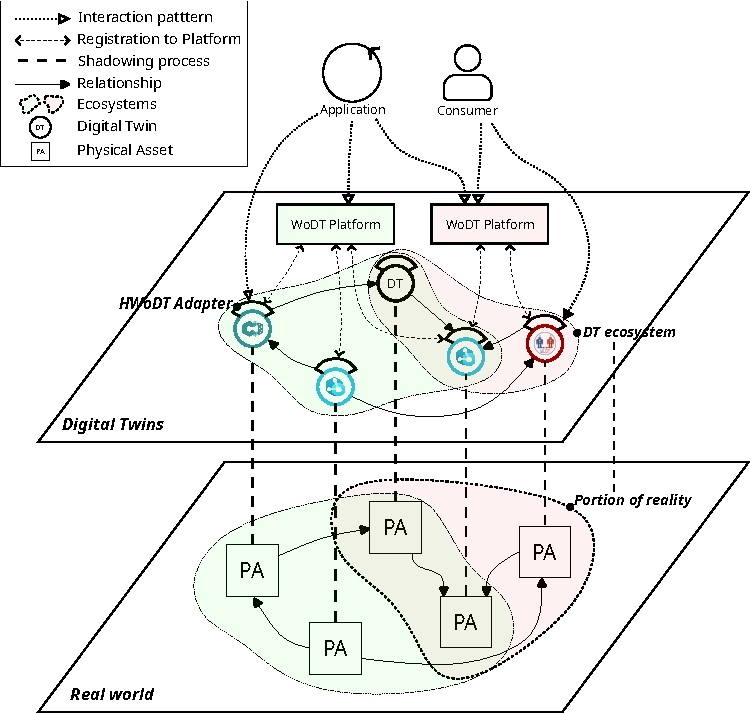
\includegraphics[width=0.7\columnwidth]{figures/hwodt/hwodt.pdf}
  \caption{The Hypermedia WoDT scheme, in the real world PAs (squares) belonging to different organizations and domains are connected by relationships. In the digital world, cross-domain ecosystems of DTs (circles) mirror different portions of reality, supported by the WoDT Platform.}
  \label{fig:hwodt}
\end{figure}

%-----------------------------------------------------------
\subsection{A Uniform Interface for Heterogeneous DTs}
\label{ssec:uniform-interface}
%-----------------------------------------------------------

The first step towards integrating heterogeneous \acp{DT} is to look into how each individual \ac{DT} can expose a uniform interface, compliant with the requirements of the \ac{HWoDT}.
Achieving standard semantic representations of \acp{DT} is an open challenge for the \ac{DT} community.
%
In this work, adopting a pragmatic approach, the benefits of uniform semantic representations in building interoperability are demonstrated through a proposal grounded on the \ac{HATEOAS} principle of the Web architecture:
each \ac{DT} must be able to provide consumers with both \emph{data} and \emph{affordances}---i.e., action possibilities---through hypermedia representations.
This leads to distinguish two logically different representations:
\begin{itemize}
    \item a \emph{\acf{DTD}}, inspired by the \ac{WoT} \acl{TD}, to hold metadata and affordances, enabling consumers to understand the \ac{DT} model, as well as which services the \ac{DT} exposes and how to access them;
    \item a \emph{\acf{DTKG}} representing the live state of the \ac{DT}, semantically encoding domain knowledge and supporting state observation, querying, and discovering relationships between \acp{DT}.
\end{itemize}

Each \ac{DT} is further required to comply with a set of standard \emph{interaction patterns} to allow consumers to uniformly obtain and manipulate such representations for all \acp{DT} in the \ac{HWoDT}.

%.................................
\subsubsection{The \acl{DTD}}
%.................................

The \ac{DTD} serves the primary purpose of providing management metadata about a \ac{DT}, registering it within the ecosystem and describing the exposed interactions\footnote{Documentation on the structure of the \ac{DTD} schema is available on GitHub \url{https://github.com/Web-of-Digital-Twins/dtd-conceptual-model}}.

A primary concern is \emph{identification} of the \ac{DT} and the associated \ac{PA} to unambiguously distinguish them from other elements of the ecosystem.
While \acp{PA} may use domain-specific identifiers (e.g., a serial number), each \ac{DT} in a \ac{HWoDT} is identified with a persistent, globally unique \ac{URI}.
This ensures identification and accessibility of \acp{DT} as Web resources throughout their whole lifecycle.

Furthermore, to support navigation from a \ac{DT} to the ecosystem it is part of, the \ac{DTD} also links to the \ac{URI} of the ecosystem---in the prototype implementation this is a URI served by the \ac{WoDT} platform to identify the \ac{DTE}.

Other relevant metadata in the \ac{DTD} concerns the model used to represent the \ac{PA} at the digital level.
%
The \ac{WoDT} metamodel (\Cref{sec:back:dt:dte})---closely aligned with the  \ac{WoT} \ac{TD}---can describe the \ac{DT} in terms of which properties, relationships, events, and actions are available to \ac{DT} consumers. 

Finally, the \ac{DTD} presents a description of the \ac{API} that consumers can use to interact with the \ac{DT}, using hypermedia controls to describe protocol bindings for the exposed interaction patterns.
%
The \ac{DTD}, is thus aligned with \ac{REST} principles as it presents both data and controls to consumers using self-descripting messages.

Even if the \ac{DTD} may evolve with new properties or interactions when a \ac{DT} gets updated, it remains mostly static as it describes the \ac{DT}'s identity metadata and software interface, not its real-time state.

%.................................
\subsubsection{The \acl{DTKG}}
%.................................

As a \ac{DT} main responsibility is to provide an up-to-date representation of the \ac{PA} state, the \ac{DTKG} complements the \ac{DTD} by representing the live state of the \ac{DT} with a \ac{KG}.

The \ac{DTKG} by means of \ac{RDF} triples, represents:
\begin{itemize}
    \item current property values;
    \item current relationships with other \acp{DT};
    \item context-dependent available actions.
\end{itemize}
Events, generated by the \ac{DT} are excluded from this representation as they are non-persistent information handled via subscriptions.

By using \ac{RDF}, the \ac{DTKG} can represent knowledge about the \ac{DT}'s state with explicit semantics using domain-specific ontologies to support a common interpretation of \ac{DT} data.
Additionally, following the Linked Data principles~\cite{Bizer_Heath_Berners-Lee_2023}, \acp{DT} linking to other \acp{DT} through relationships supports navigating across the ecosystem in a distributed \ac{KG}.

%.............................................
\subsubsection{\acl{DT} Interaction Patterns}
%.............................................

Other than generating the necessary \ac{DTD} and \ac{DTKG} each \ac{DT} in a \ac{HWoDT} ecosystem is required to implement a Web \ac{API} for consumers. This enables direct use by any Web client.

First, the \ac{API} should expose methods to retrieve the two \ac{DT} representations presented above.
%
As the main function of a \ac{DT} is to represent the \ac{PA} state over time, when dereferencing the \ac{URI} which identifies the \ac{DT} with an HTTP GET request the \ac{DT} must return the current \emph{snapshot} of the \ac{DTKG}.

\begin{figure}
    \centering
    \begin{subfigure}[t]{0.45\columnwidth}
        \centering
        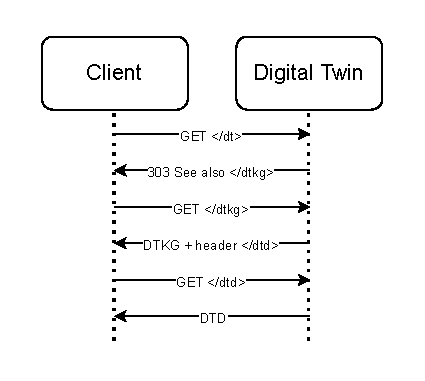
\includegraphics[width=\textwidth]{figures/hwodt/dtddtkg.pdf}
        \caption{}
        \label{fig:sequence-dtddtkg}
    \end{subfigure}
    \hfill
    \begin{subfigure}[t]{0.46\columnwidth}
        \centering
        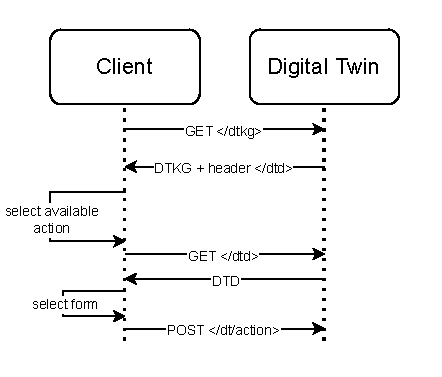
\includegraphics[width=\textwidth]{figures/hwodt/dtdactioncrop.pdf}
        \caption{}
        \label{fig:sequence-action}
    \end{subfigure}
    \caption{Interaction patterns to (a) access the \ac{DTD} and \ac{DTKG} and (b) invoke available actions on a \ac{DT} through the uniform interface and standard Web patterns.}
    \label{fig:sequence-interactions}
\end{figure}



Technically, since a \ac{DT} qualifies as a \emph{non-information resource}\footnote{For a discussion on information vs. non-information resources see \url{https://www.w3.org/TR/cooluris/} and \url{https://lists.w3.org/Archives/Public/www-tag/2005Jun/0039.html}}
the standard Web practice is returning a 303 (See Other) status code with the \textit{Location} HTTP header set to the \ac{URL} of the \ac{DTKG} information resource.
%
The \ac{URL} of the \ac{DTD} is linked in an HTTP Link Header with a custom relation type \texttt{dtd} in the response of the \ac{DTKG} GET request.
%
In this way, consumers can follow links between resources and access both \ac{DT} representations with standard Web interactions as shown in \Cref{fig:sequence-dtddtkg}.

Since the \ac{DTKG} evolves over time to reflect the \ac{PA} state, \acp{DT} are required to support a subscription \ac{API} to observe such changes (e.g., via WebSockets, long-polling, or WebSub~\cite{websub}).
Modeling the \ac{DTKG} as a Web resource also enables basic historicization using protocols like Memento~\cite{rfc7089}, if the \ac{DT} acts as a Memento TimeGate.

Finally, the \ac{API} may expose \ac{DT} actions that can be invoked by external consumers.
The \ac{DTKG} shows which actions are currently valid, while the \ac{DTD} describes how to request their execution to the \ac{DT}.
Consumers rely on both to interact and invalid actions should fail (e.g., with HTTP 403), ensuring consistency with the \ac{DT} model.
%
Figure \ref{fig:sequence-action} illustrates the interaction pattern to invoke an action on a \ac{DT}, by first checking its availability in the \ac{DTKG} and then following the affordance described in the \ac{DTD} to execute it.

%---------------------------------------------
\subsection{Ecosystem Services in the HWoDT}
\label{ssec:ecosystem-services}
%---------------------------------------------

In the proposal for realizing the \ac{HWoDT} ecosystem functionalities described in \Cref{chap:dte:dte} are implemented through a middleware:
%
the \emph{\ac{WoDT} Platform} aggregates data from registered \acp{DT} and exposes an \ac{API} that consumers can use to manage and interact with the ecosystem as a whole.

%........................................
\subsubsection{Managing the \acl{HWoDT}}
%........................................

The \ac{HWoDT} proposal assumes that \acp{DT} are existing, independently running software entities which implement the uniform interface presented in \Cref{ssec:uniform-interface}.
%
Hence, the \ac{DT} creation is handled by developers with their technology of choice, and adding it to an ecosystem is simply a matter of registering it to a \ac{WoDT} Platform. 
%
The platform exposes an \ac{API} that either managers, an external service or a \ac{DT} itself, can use to submit a \ac{DTD} to register a new \ac{DT} to the ecosystem.
The \ac{DTD} is then stored in a registry, which further allows it to be updated or removed if the \ac{DT} leaves the ecosystem.
%
Consumers can also use the registry \ac{API} to discover which \acp{DT} are in the ecosystem and to filter them based on metadata in the \ac{DTD}---e.g., they can discover if multiple \acp{DT} in the ecosystem model the same \ac{PA} filtering on the \ac{PA} identifier.

These simple operations are sufficient to manage the ecosystem. 
%
The \ac{DTD} is used in the registration process as it provides the necessary metadata to assess membership and compliance requirements as well as the \ac{API} description that the platform can use to interact with the \ac{DT} upon registration.
% 
Once registered, the platform uses the \ac{API} description within the \ac{DTD} to access and observe the \ac{DTKG}.  
It can also notify successful registration, enabling the \ac{DT} to record the platform \ac{URI} in its list of ecosystems updating its \ac{DTD} accordingly.

%..........................................
\subsubsection{Exploiting the \acl{HWoDT}}
%..........................................

By observing each individual \ac{DTKG}, the platform can cache the latest update and aggregate them to create a global \ac{DTE} \ac{KG} that can be exploited to implement ecosystem-level services for consumers.
%
The \ac{DTD} and \ac{DTKG} of each \ac{DT} are stored within the \ac{KG}, allowing queries to easily retrieve all available information about a \ac{DT}.
%
Each update of a \ac{DTKG} is processed and merged in the global \ac{KG} so that current representation of the whole ecosystem is always available to consumers.



The \ac{DTE} is a non-information resource and has a \ac{URI} which, when dereferenced, returns the global \ac{DTE} \ac{KG}\footnote{As the ecosystem \ac{KG} can be very large, returning the whole thing can be impractical. Alternatives include returning a partial representation with links to the \acp{DT} caches}.
%
Consumers can also \emph{query} the \ac{DTE} \ac{KG} through the \ac{WoDT} platform SPARQL endpoint.
%
This enables the extraction of selected information from the current state of all \acp{DT} in the ecosystem with a standard query language.

Finally, consumers may want to observe the evolution of the ecosystem \ac{KG}. The platform must then support an \ac{API} to receive subscription requests and send updates to observers.
%
Given the large nature of the \ac{DTE} \ac{KG}, consumers might not be interested in receiving \emph{all} updates. Hence, techniques for \ac{RDF} stream processing~\cite{barbieri2009www} might be more effective to support selective observation.

%======================================================
\section{A Prototype Framework for the HWoDT}
\label{sec:hwodt-impl}
%======================================================

To support the prototyping of heterogeneous \acp{DTE} based on the \ac{HWoDT} proposal, a set of tools is implemented aiming at the integration of existing \ac{DT} technologies.
%
The HWoDT framework is open source and available on GitHub\footnote{\url{https://github.com/Web-of-Digital-Twins}}. 

The software distribution includes a prototype \emph{\ac{WoDT} Platform} implementation and \emph{adapters} to implement the \ac{HWoDT} uniform interface for \acp{DT} developed with \azureTwin{}, \ditto{}, and the \ac{WLDT} framework (\Cref{sec:dte:engineering-dt:wldt-framework}).
%
The technology choice is meant to be representative of the state of the art as they differ in terms of functionalities, namely \azureTwin{} is a cloud platform, Ditto is an open-source platform, and \ac{WLDT} allows developing and deploying \acp{DT} as standalone software processes.
This section presents the overall architecture (\Cref{fig:abstract_arch}) and its implementation.


\begin{figure}
  \centering
  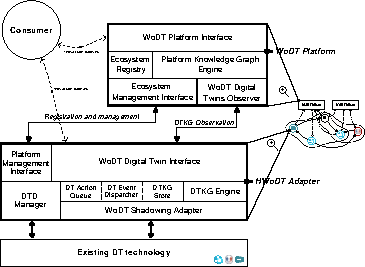
\includegraphics[width=0.8\columnwidth]{figures/hwodt/abstract_arch.pdf}
  \caption{Overall abstract architecture of the \ac{HWoDT} framework, showing the main functional modules. On the bottom existing \acp{DT} which, through the adapter, can implement the \ac{HWoDT} uniform interface and be integrated with a \ac{WoDT} platform.}
  \label{fig:abstract_arch}
\end{figure}



%----------------------------------------------
\subsection{A WoT-compatible \acl{DTD}}
%----------------------------------------------

The \ac{DTD} is a central component in the design of the uniform interface of the \ac{HWoDT}.
%
Its design is inspired to the \ac{WoT} \ac{TD}, as an \ac{API} description of the functionalities offered by a \ac{DT}.

Although the \ac{WoT} explicitly reference \acp{DT} in its architectural patterns, the \ac{TD} alone does not support all the metadata that are needed in the proposed \ac{DTD}.
Hence, using \ac{WoT}-compliant mechanisms, \acp{TD} are extended to include the relevant metadata in order to qualify as a functional \ac{DTD} for a prototype implementation of the \ac{HWoDT}.
%
Namely, the \ac{TD} is extended using a custom \emph{\ac{WoDT} vocabulary}\footnote{\url{https://github.com/Web-of-Digital-Twins/wodt-vocabulary}}
which defines concepts to implement the \ac{DTD} and the \ac{DTKG}, as well as HTTP Link Headers relation types used in the interactions of the \ac{HWoDT} (see \Cref{ssec:uniform-interface}).
%
\Cref{lst:dtd-thing-model} shows a generic \ac{TM}~\cite{wot-td} that can be used to implement a valid \ac{DTD}. The \ac{DTD} must include:
\begin{itemize}
    \item the \ac{PA} identifier, 
    \item a link to the \ac{DTKG},
    \item an \texttt{observeallproperties} affordance to subscribe to updates of the \ac{DTKG}.
\end{itemize}

\lstinputlisting[
    label={lst:dtd-thing-model},
    caption={The Thing Model that Thing Descriptions must
    implement to be recognized as a valid \acl{DTD}.},
]{listings/hwodt/dtd.jsonld}


% \begin{figure}
%   \centering
%   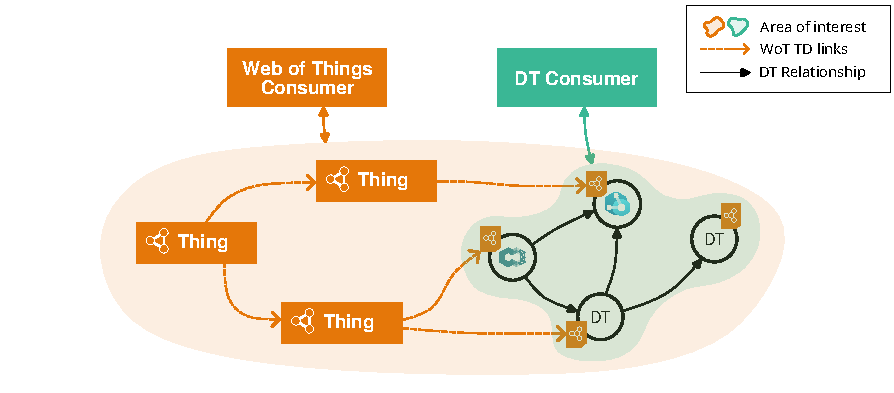
\includegraphics[width=\columnwidth]{figures/hwodt/wot-dt-mashups.pdf}
%   \caption{Keeping Digital Twin representations aligned with the \ac{WoT} Thing Description enables the creation of mixed mashups and interoperability with existing \ac{WoT} consumers.}
%   \label{fig:wot-dt-mashups}
% \end{figure}

The alignment with the \ac{WoT} is strategic for the \ac{DT} community as reusing the existing standard ensures compatibility and favors the development of application mashups.
%
The \ac{DTD} can be served by the \ac{DI} of a \ac{DT} to be discovered and consumed by existing \ac{WoT} clients (see \Cref{sec:dte:engineering-dt:physical-digital-adapters}).
%
Clients that have the capability to interpret the \ac{WoDT} vocabulary can then exploit the additional metadata to interact with the \ac{DT} as part of a \ac{HWoDT} ecosystem as shown in \Cref{fig:wot-dt-mashups}.

%-----------------------------
\subsection{HWoDT Adapters}
\label{ssec:adapters}
%------------------------------

\acp{DT} in a \ac{HWoDT} ecosystem must all adhere to the uniform interface, regardless of the technology used to implement them.
%
Adapting existing \ac{DT} technologies to the \ac{HWoDT} interface requires aligning data and interaction patterns.
%
To show that this alignment is achievable with configurable reusable components a set of \emph{adapters} is developed to integrate some mainstream technologies within a \ac{HWoDT} ecosystem.
%
All adapters support HTTP interactions and WebSocket-based \ac{DTKG} observation.
%
The abstract architecture followed by all adapters is shown in \Cref{fig:abstract_arch}, bottom.

%..............................................
\subsubsection{\azureTwin{} Adapter}
%..............................................

\azureTwin{} is Microsoft's domain-independent \ac{PaaS} \ac{DT} solution, supporting the management of multiple \acp{DT} connected within a \emph{twin graph}.

Creating \acp{DT} in \azureTwin{} requires defining their model using the \emph{\acf{DTDL}}, a custom JSON-LD format to specify properties, relationships, commands (actions) and telemetry (events) that describe a \emph{type} of \ac{DT}.
%
\ac{DTDL} models can then be used to create \ac{DT} instances.
%
Although the model closely aligns with the \ac{WoDT} model, the support of events and actions is partial\footnote{As of June 2025, commands can be defined but not invoked automatically, while telemetries are not used within \azureTwin{} \url{https://learn.microsoft.com/en-us/azure/digital-twins/concepts-models}} and relationships are limited to linking \acp{DT} within the same \azureTwin{} instance, which hence defines a closed homogeneous ecosystem.

The \azureTwin{} adapter is implemented as a middleware, connecting to an \azureTwin{} instance and mapping \acp{DT} to the \ac{HWoDT} uniform interface.
%
The adapter can be configured to select which \acp{DT} needs to be mirrored and specify the mapping from \ac{DTD} properties and relationships to produce the \ac{DTKG}. 
%
\Cref{fig:azure-adapter-c&c} shows the adapter architecture and the necessary components to connect to an \azureTwin{} instance.
%
The following Azure service pipeline must be set up to link the \azureTwin{} instance to the adapter:
\begin{itemize}
    \item \textit{Azure Event Grid} to capture and forward \azureTwin{} events;
    \item \textit{Azure Function} (\acl{FaaS}) to fetch the current \ac{DT} state and send it to the adapter via SignalR on every new event;
    \item \textit{Azure SignalR} to deliver \acp{DT} state updates to the adapter.
\end{itemize}

The adapter can be deployed either within the Azure cloud or is designed to automatically retrieve the \ac{DTDL} models, stored on \azureTwin{}, and convert them in valid \acp{DTD} for each \ac{DT} instance.
The adapter waits for SignalR events to receive \ac{DT} state updates generated by the Azure Function and convert them into \acp{DTKG} updates.

\begin{figure}
    \centering
    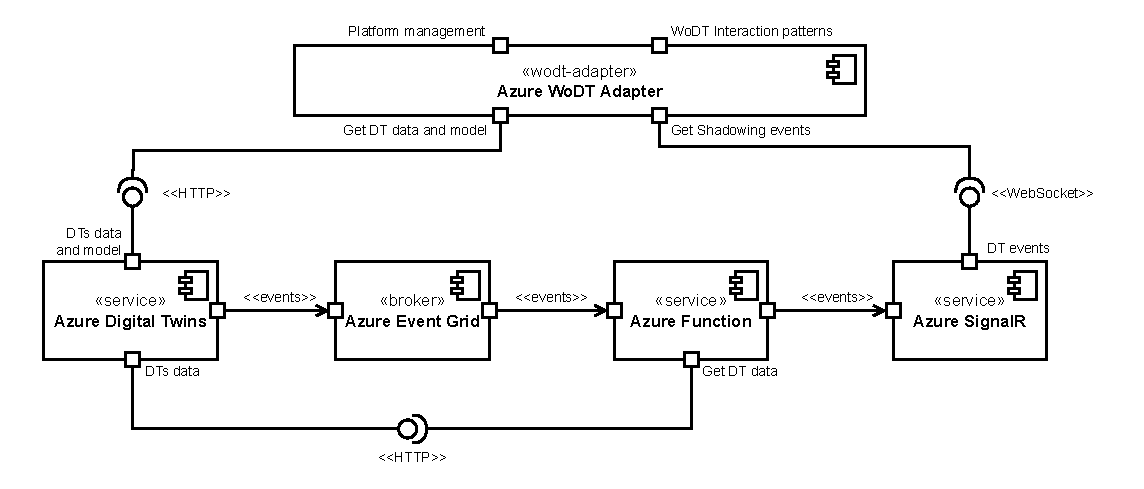
\includegraphics[width=\textwidth]{figures/hwodt/adtadapter-c&c.pdf}
    \caption{The \azureTwin{} adapter, implemented as a standalone component that maps specific instances of \acp{DT} hosted on an \azureTwin{} instance.}
    \label{fig:azure-adapter-c&c}
\end{figure}

%..............................................
\subsubsection{Eclipse Ditto Adapter}
%..............................................

\emph{Eclipse Ditto}, is an open-source \ac{DT} platform from the Eclipse Foundation. 
It abstracts each \ac{PA} as a \emph{Ditto Thing} and offers a Web-based layer for interacting with \ac{IoT} devices through their \acp{DT}.
%
A Ditto instance can manage multiple \acp{DT}, using a metamodel with:
\begin{itemize}
    \item \emph{Attributes} for static metadata,
    \item \emph{Features} which can group data (properties) and functionalities (messages).
\end{itemize}
Although lacking native support for relationships, actions, and events, these can be modeled using attributes (for links), consumer-to-\ac{DT} messages (for actions), and \ac{DT}-to-consumer messages (for events). Models can be defined via a custom JSON format or a (set of) \ac{WoT} \ac{TM}.

Eclipse Ditto is implemented with a microservice architecture. 
Despite Ditto being open-source and allowing the development of custom extensions, the prototype adapter is implemented as a custom external middleware that can be deployed to map one Ditto Thing to the \ac{HWoDT} uniform interface.
%
The middleware leverages Eclipse Ditto's native WebSocket interface to retrieve data and performs two key transformations: converting the \ac{WoT} \ac{TD} exposed by Ditto into a \ac{DTD}, and serializing \ac{DT} data into a \ac{DTKG}.
This process relies on a configurable mapping between Ditto features and their corresponding \ac{RDF} representations.

\begin{figure}[ht]
  \centering
  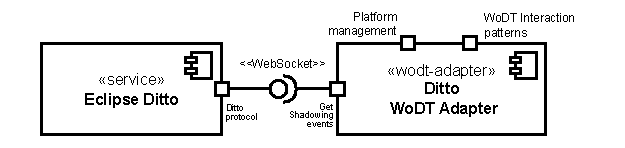
\includegraphics[width=0.8\columnwidth]{figures/hwodt/ditto-adapter-c&c.pdf}
  \caption{The Eclipse Ditto adapter, implemented as a standalone component that maps a specific instance of a \ac{DT} hosted on the Ditto platform.}
  \label{fig:ditto-adapter-c&c}
\end{figure}

%..............................................
\subsubsection{\acl{WLDT} Adapter}
%..............................................

The \emph{\acf{WLDT} framework} (\Cref{sec:dte:engineering-dt:wldt-framework}) enables the development of \acp{DT} as standalone software components deployable across cloud or edge environments.
%
Specifically, the adapter is implemented as a \ac{DiA}, used in the \ac{WLDT} architecture to represent digital interfaces through which the \ac{DT} can expose data for consumers.
%
The framework internal metamodel is already aligned with the \ac{HWoDT}, so no additional effort is required to map concepts.
The adapter is provided as a reusable Java library, which \ac{WLDT} developers can easily import into their projects and then configure the mapping towards the \ac{HWoDT} uniform interface leveraging the implementation of the necessary \ac{API} to manage the \ac{DTD} and \ac{DTKG}.

\begin{figure}[ht]
  \centering
  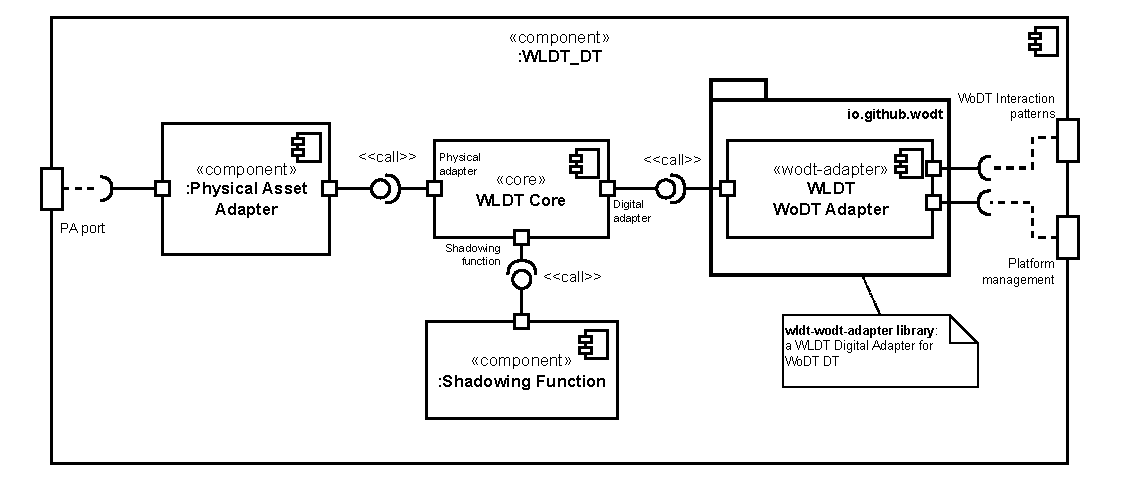
\includegraphics[width=\textwidth]{figures/hwodt/wldt-adapter-c&c.pdf}
  \caption{The architectural diagram of the \ac{WLDT} adapter, illustrating its integration with the other components of the framework.}
  \label{fig:wldt-adapter-c&c}
\end{figure}


%..............................................
\subsubsection{Implementing Custom Adapters}
%..............................................
The description of the adapters implemented in the prototype \ac{HWoDT} framework should be useful for any \ac{DT} developer wishing to implement a custom adapter for their own \ac{DT} or \ac{DT} technology. 
%
The idea of the \ac{HWoDT} is grounded on the fact that implementing such custom adapters is relatively straightforward and that the little effort spent in developing (or even less in configuring) them can bring benefits in the integration with the \ac{HWoDT} ecosystem.

To summarize, the steps to develop a custom adapter are: 
\begin{enumerate}
    \item understand how to map the concept of the original \ac{DT} model into the \ac{WoDT} metamodel;
    \item understand how to represent the state of the \ac{DT} with an evolving semantic representation for the \ac{DTKG};
    \item implement a module that can reactively produce the \ac{DTKG} whenever the \ac{DT} state is updated;
    \item implement a module that can serve the \ac{DTD} over HTTP, alongside the mandatory \ac{API} for \ac{DTKG} observation.
\end{enumerate}

%-----------------------------------
\subsection{The WoDT Platform}
%-----------------------------------

A prototype of a \ac{WoDT} Platform is implemented in Kotlin.
The platform implements the modules of the abstract architecture shown in \Cref{fig:abstract_arch}, top as shown in \Cref{fig:platform-c&c}.
%
Namely, the platform offers multiple interfaces for consumers: an HTTP \ac{API} for \ac{DTE} management (Ecosystem Management Interface) and one for \ac{KG} access with a SPARQL endpoint for read-only queries, as well as a WebSocket endpoint to observe ecosystem updates (\ac{WoDT} Platform Interface).

The platform can process the \ac{WoT}-based \ac{DTD} described above to register \acp{DT}.
When a registration requested is submitted, the platform:
\begin{enumerate}[label=\textbf{Step \arabic*}, leftmargin=5.3em]
    \item locates the \ac{DTKG} observation form (\texttt{observeallproperties}) and starts observing the \ac{DT} for updates;\label{step:observe-dtkg}
    \item notifies the \ac{DT} of successful registration to let it update its \ac{DTD} with the platform URI;\label{step:notification}
    \item maps the \ac{DT} \ac{URI} to a local cache URL;
    \item observes \ac{DTKG} updates and merges them into the \ac{DTE} \ac{KG} stored in memory with Apache Jena.
\end{enumerate}

%
The current prototype supports the observation of \ac{DTKG} through WebSockets for \ref{step:observe-dtkg} and implements \ref{step:notification} sending a request to a hardcoded \texttt{/platform} HTTP endpoint on the \ac{DT}.

Consumers can interact with the \acp{DTE} through the \ac{WoDT} platform
either through (possibly repeated) SPARQL queries to retrieve the information they need or by observing the whole \ac{KG} through WebSockets.
%
In the prototype, all observers receive the whole \ac{KG} whenever there is an update so that consumers don't need to have specific update handling logic.
%

\begin{figure}
  \centering
  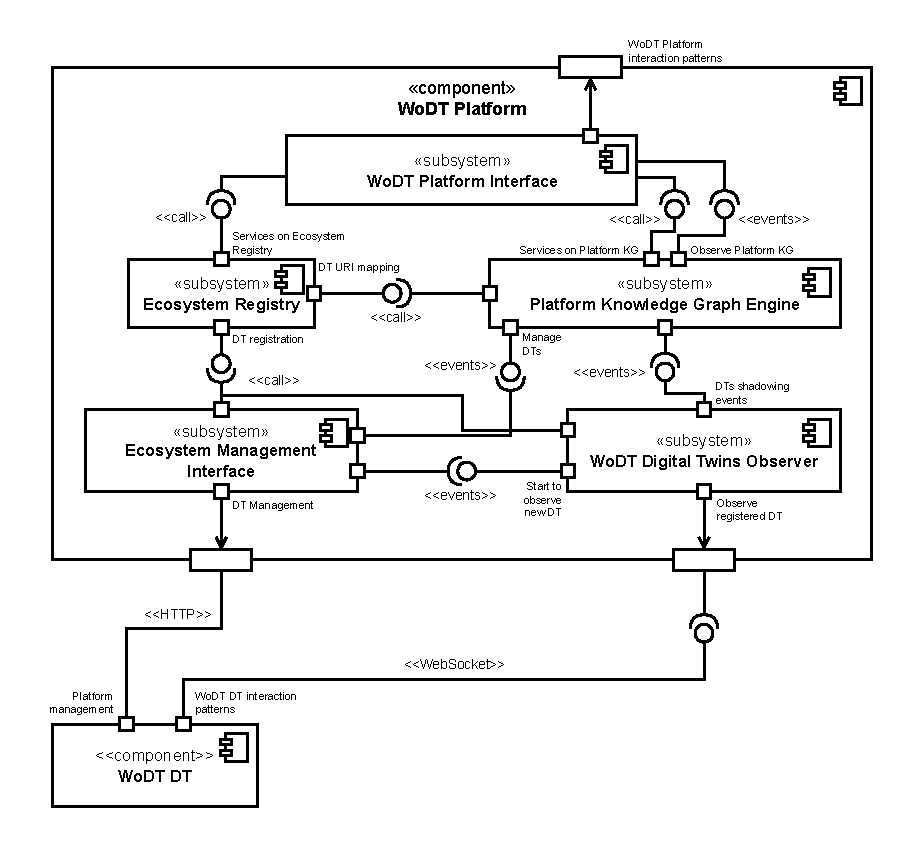
\includegraphics[width=\columnwidth]{figures/hwodt/platform-c&c.pdf}
  \caption{\ac{WoDT} Platform modules and interfaces, represented using components and connectors.}
  \label{fig:platform-c&c}
\end{figure}


%=======================================
\section{Comparison with Related Works}
%=======================================

This section compares the \ac{HWoDT} proposal with related approaches that target the integration of \acp{DT} in ecosystems. 
%
The aim of this comparison is to highlight the similarities and differences with existing solutions, discussing advantages and limitations of existing approaches with respect to the \ac{HWoDT}.

The \ac{HWoDT} proposal is not meant to compete with existing standards or framework, but rather to either complement them or provide an alternative approach to \ac{DT} interoperability.
%
The main principle of the \ac{HWoDT} is to promote interoperability through the adoption of \ac{REST} principles and Semantic Web technologies, given their proven effectiveness in enabling integration across heterogeneous systems on the Web.


%----------------------------------------------------
\subsection{HWoDT vs. Industrial Standards}
%----------------------------------------------------

The \ac{HWoDT} tackles the relevant issue of enabling \ac{DT} interoperability targeting the creation of \emph{heterogeneous \acp{DTE}}.
%
This is an open challenge in the \ac{DT} research community (see \Cref{sec:back:dt:interoperability}), and several interoperability frameworks are being proposed to streamline the integration of \acp{DT}~\cite{Barnard_2024}.
%
Among the most relevant standards some of the most relevants are \ac{OPC-UA}, \ac{AAS}, \ac{AML} and the \ac{W3C} \ac{WoT}. \Cref{tab:interop_comparison} summarizes a comparison of these standards across selected aspects.

Given the different nature of these standards, they can be viewed as complementary rather than competing against each other.
%
There have been integration efforts in order to leverage their different strengths. For instance, \ac{OPC-UA} has been integrated with web technologies~\cite{DBLP:journals/csi/CavalieriSS19} to support direct integration with web clients, operations in \ac{AAS}~\cite{platform_i40_aas_part1_v2} and affordances in \ac{WoT}\footnote{\url{https://profiles.opcfoundation.org/workinggroup/97}} can have an \ac{OPC-UA} protocol bindings, and \ac{AML} specifications can be linked to \ac{AAS} to have a coherent view of the involved assets~\cite{DBLP:conf/etfa/DrathRH19,DBLP:conf/indin/WengerZ018}.
%
In this view, the Semantic Web technologies adopted in the \ac{HWoDT} approach can be integrated on top of existing standards and complement their features.

\begin{table*}
    \centering
    \small
    \setlength{\tabcolsep}{3pt} % reduce inter-column spacing
    \renewcommand{\arraystretch}{1.3} % slightly tighter rows
   \begin{tabular}{>{\raggedright\arraybackslash}p{2cm}|>{\raggedright\arraybackslash}p{2.2cm}|>{\raggedright\arraybackslash}p{2.2cm}|>{\raggedright\arraybackslash}p{2.2cm}|>{\raggedright\arraybackslash}p{2.2cm}|>{\raggedright\arraybackslash}p{2.2cm}}
    \toprule
    \midrule
    \textbf{} & \textbf{AAS} & \textbf{OPC-UA} & \textbf{AML} & \textbf{WoT} & \textbf{Semantic Web} \\
    \hline
    \hline
    \textbf{Scope} &
    Asset digital representation &
    Device data / \ac{M2M} &
    Tool interoperability &
    Web-scale access &
    Cross-domain knowledge \\
    \hline
    \textbf{Data model} &
    Submodels + semantic IDs &
    Hierarchical node graph (address space) &
    Hierarchies (CAEX, CAD, PLCopen) &
    Thing Description (JSON-LD) &
    Triple Graphs (RDF / OWL) \\
    \hline
    \textbf{Semantics} &
    Structured submodels, semantic references &
    (Sub)Types and Relationships &
    Role-based, structural  &
    JSON-LD semantics, ontology-aligned &
    General-purpose ontologies \\
    \hline
    \textbf{Querying and Data access} &
    REST API &
    Browse address space &
    File access &
    SPARQL (if RDF-mapped) &
    SPARQL / Web browsing \\
    \hline
    \bottomrule
    \end{tabular}
    \caption{Comparison of interoperability frameworks across selected aspects.}
    \label{tab:interop_comparison}
\end{table*}


The Semantic Web excels at general-purpose knowledge representation, and integration of such heterogeneous knowledge under a uniform interface (\Cref{sec:back:web:semantic-web-technologies}).
%
Additionally, it enables reasoning through ontological inference and expressive queries across concepts, supporting use cases that have limited support when using the aforementioned standards alone (see \cref{tab:interop_comparison}, Querying and Data access).
%
It is then not surprising that alignment between Semantic Web technologies and industrial standards are being investigated, highlighting similarities between e.g., \ac{OPC-UA}~\cite{DBLP:conf/etfa/MajumderWD19,DBLP:conf/etfa/PerzyloP0K19} and \ac{AAS}~\cite{DBLP:conf/icphys/BedenCB21, platform_i40_aas_part1_v2} data models, to benefit from these features.

The \ac{HWoDT} proposal, follows this trend, suggesting that the hypermedia layer can serve as an integration on top of existing \acp{DT}, which may already have an implementation based on industrial standards.
%
Additionally, since the described interoperability standards emerged from the Industry 4.0 movement, they generally target only industrial domains. This poses a significant gap when needing to map concepts and represent entities from different domains.
%
The \ac{HWoDT} approach, addresses this gap through the use of Web ontologies which have been developed for a high variety of application domains and can be seamlessly integrated within the same \ac{KG}.

Finally, providing a synchronized representation is a key feature of \acp{DT}.
The \ac{HWoDT} approach, designed with a \ac{DT}-centric perspective, requires each \ac{DT} to produce and update such representation of its current state through the \ac{DTKG}. This supports consumers in both querying an up-to-date view of the whole ecosystem and observing changes on the \ac{DT} state.
%
Similar behavior can be implemented by \ac{AAS} servers (e.g. Eclipse BaSyx\footnote{\url{https://eclipse.dev/basyx/}}) that automatically retrieve data from \ac{OPC-UA} endpoints, but is limited by the expressiveness of queries on the \ac{AAS} model typically relying on Web APIs with no hypermedia support.

Overall, the comparison shows that the \ac{HWoDT} approach is compatible and complementary to existing \ac{DT} interoperability efforts and follows existing research directions aimed at bridging the Semantic Web on top of industrial standards.
The approach can be used as an additional layer integrating \acp{DT} implemented with (or without) other standards to support:
\begin{itemize}
    \item integration with \acp{DT} outside the industrial domain,
    \item advanced query with reasoning on semantic structures,
    \item simple Web-based navigation and direct access to the up-to-date representation of the mirrored asset,
    and 
    \item subscription to changes in the \ac{DT} state.
\end{itemize}

%-------------------------------------
\subsection{HWoDT vs. WoT mashups}
%-------------------------------------

Leveraging the \ac{HWoDT}, developers can focus only on application logic, abstracting away the complexity of heterogeneous \ac{DT} integration.  
This yields two important advantages that are shared with the \ac{WoT} approach:  
\begin{inlinelist}
    \item the application layer is more stable as it remains unaffected by the introduction of new \acp{DT};
    and  
    \item the \ac{DT} layer can evolve or replace underlying implementations without affecting upper layers as long as the exposed interface is not changed.
\end{inlinelist}

Still, a fundamental difference between the \ac{HWoDT} and the (semantic) \ac{WoT} is the ability to seamlessly browse a \ac{KG} of the \ac{DTE} that captures explicitly the \acp{DT}' observable state. 
%
In a W3C \ac{WoT} application, even if \acp{TD} were to be semantically annotated and stored in a \ac{KG}, selecting \emph{things} based on their state properties would require sending the necessary requests to retrieve the current value of each property of each thing.
%
This is because the W3C \ac{WoT} is not tailored to the requirements of \acp{DT}, which, instead, are by definition capable of shadowing---and thus to always show the current state of the asset they represent.
%
Furthermore, the W3C \ac{WoT} does not specify how to handle dynamic relationships between things, limiting the possibility of expressing powerful queries on the state of interrelated assets.
%
The \ac{HWoDT} proposal, leverages this \ac{DT}-specific feature through the \ac{DTKG} component, simplifying the interaction. 
%
Similarly, even when dealing with a set of heterogeneous \acp{DT}, without the unifying abstraction of the \ac{HWoDT}, consumers would need to retrieve the \ac{DT} state representation from each individual \ac{DT}, interpret them and merge the data to resolve the query (\Cref{fig:comparison-custom-vs-hwodt}).

\begin{figure}
  \centering
  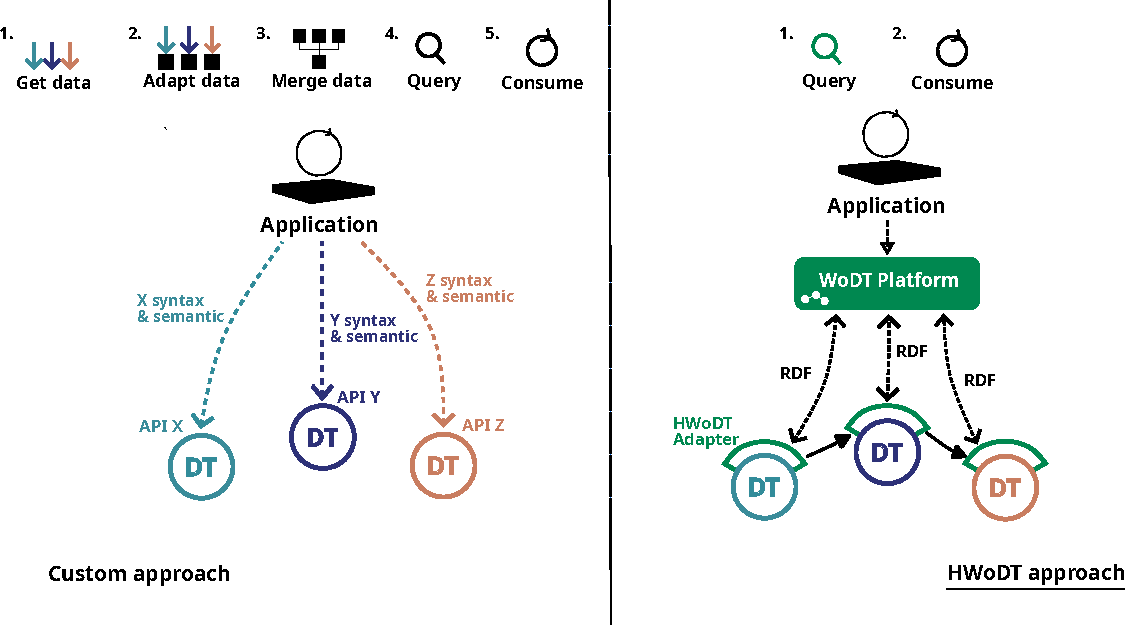
\includegraphics[width=\columnwidth]{figures/hwodt/comparison_custom_hwodt.pdf}
  \caption{Comparison of the steps required to perform a ``query'' across heteregenous \acp{DT} versus with the \ac{HWoDT} approach, which abstracts heterogeneity through a uniform interface.}
  \label{fig:comparison-custom-vs-hwodt}
\end{figure}

%-------------------------------------------------------
\subsection{HWoDT vs. Closed DT Platforms}
%-------------------------------------------------------

The \ac{HWoDT} approach, offers a solution to implement open \acp{DTE} on top of heterogeneous \ac{DT} technologies.
%
This contrasts with the vision of other \ac{DT} platforms which, instead, support homogeneous \acp{DTE} and offer support for the definition of multiple \acp{DT} within the same instance, but constraining all of them to adhere to specific technological choices.

The most recognized technology for building \acp{DTE} is the off-the-shelf solution offered by \acl{ADT}.
The graph-based rationale within the platform has been an inspiration for the \ac{HWoDT}, as a way to connect multiple \acp{DT} and obtain a cohesive view of the physical reality.

Still, \acl{ADT} is a Platform-as-a-Service solution, only available through the Azure cloud, strongly limiting its application in different scenarios where the \acp{DTE} might be constructed on a private infrastructure.
%
The technological stack is completely custom, creating a vendor lock-in on the developed \acp{DT} models.
% 
Azure requires \acp{DT} to be defined using its own custom \ac{DTDL}, supports only custom ontologies (or requires converting existing ones form \ac{OWL} to \ac{DTDL}) and supports queries on the \emph{twin graph} only through a custom SQL-like query language.
%
Furthermore, in closed approaches, it would not be possible to create relationships with entities that are outside of the supporting platform. For instance, the relationship model of \azureTwin{} requires to define possible relationships between \ac{DTDL} models.
%
The \ac{HWoDT} addresses this limitation by enabling the definition of cross-platform \ac{DT} relationships using Linked Data principles.   
This enhances the expressiveness of \acp{DTE} and allows developers to model ecosystems that more accurately reflect domain knowledge.

Through the \ac{HWoDT} we reclaim the vision of open \acp{DTE} that can be enabled by a stack of open standards and technologies. 
%
This offers an alternative to closed platforms, allowing the development of \acp{DTE} in a variety of different settings tailored to the specific use case needs.

Although open-source \ac{DT} platforms like the aforementioned Eclipse Ditto exist, they have not being designed with an ecosystem perspective in mind. 
Differently from the \ac{HWoDT}, platforms like Ditto merely support having multiple instances of \acp{DT} hosted on the same platform and exposing similar \ac{API}. 
%
This constraints the \ac{DT} implementation to adhere to Ditto models, protocols and \ac{API}, does not offer native support for tracking meaningful dynamic relationships between assets and has very limited query capabilities\footnote{Ditto supports queries through a search \ac{API} based on the Resource Query Language \url{https://eclipse.dev/ditto/basic-search.html}}


%-------------------------------------------------------
\subsection{HWoDT vs. Other Web-based DTs}
%-------------------------------------------------------


The \ac{HWoDT} is not the first attempt to leverage Web features in \acp{DT} implementations. Service-oriented and micro-service architectures are among the most prominent architectural patterns when it comes to implementing \acp{DT} according to a recent survey~\cite{ferko2022architecting}, making a strong parallel with Web services.

In \cite{Liu_Jiang_Jiang_2020} the authors propose a Web-based approach for the development of \acp{DT} of a production system.
They leverage a multi-layer architecture with the uppermost layer exposing \ac{REST} \acp{API} and ontologies to describe the components of a \ac{CPS} using the abstraction of production nodes.
%
Although the approach shares some similarities with the \ac{HWoDT} proposal in enabling a uniform interface to organize modules of a \ac{CPS}, it is heavily restricted to the manufacturing domain and, crucially, it relies on all the production nodes to use the same technological stack and does not include heterogeneous \acp{DT}.

In \cite{Autiosalo_Siegel_Tammi_2021} the authors propose an approach for a \emph{Digital Twin Web} and an open-source implementation of a Web server to host \ac{DT} description documents called Twinbase through Git-based workflows.
%
The approach shares the main motivations that are behind the \ac{HWoDT} proposal, leveraging Web standards to promote interoperability and connect \acp{DT} in a network that any consumer can access with a Web browser. The main goal is to provide a meta-level registry of \acp{DT} so that consumers can discover them and also shares the idea of having relationships between \ac{DT} instances.
%
Despite these similarities, the approach differs for several reasons. First, the proposed description is not using any semantics, enforcing a very basic model for representing the \acp{DT} using Yaml files. Second, the represented \acp{DT} are mostly static, and do not share their state in a uniform way but only link to other resources or \acp{API} to interact with the \ac{DT} state under a set of generic \emph{features} the \ac{DT} can expose. Third, the proposed architecture based on Git workflows is limiting to a very specific subset of applications that can deal with that kind of interface to publish updates.

Finally, other approaches exploit the \ac{WoT} in the context of \acp{DT}. In this work, the \ac{WoT} \acp{TD} is semantically extended to implement a preliminary \ac{DTD}. 
%
A similar extension is presented in \cite{González-Gerpe_Cimmino_Bernardos_Poveda-Villalón_García-Castro} which proposes to use the \ac{TD} ontology in the construction domain, extending it to capture the five-dimensional model of \acp{DT}~\cite{qi2021enablingtechdt}.
%
The \ac{WoT} is also the foundation of WoTwins~\cite{SciulloWoTwins2022} a framework to generate automatically \acp{DT} starting from existing \ac{WoT} things, modeling their behavior and enabling prediction features. 
%
These works highlight the relevance of the \ac{WoT} as a standard for the future of \ac{DT} applications, despite its limitations in capturing fully the nature of a \ac{DT} in its entirety which may require extensions and development of custom ontologies aligned with the \ac{WoT} model.

%==========================================
\section{Prototype Performance Evaluation}
%==========================================

A performance evaluation of the prototype is carried out to quantify the performance implications introduced by the additional layer introduced by the \ac{HWoDT} to implement \acp{DTE}.
%
\Cref{fig:latency-hwodt} schematically shows the communication between components in a \ac{HWoDT}-based system. \circled{A} is the latency between \ac{PA} and \ac{DT}, \circled{B} is the latency between the \ac{DT} and the \ac{HWoDT} adapter, \circled{C} is the latency between the adapter and the platform, while \circled{D} is the latency between the platform and the client. In a scenario where the DT is used without the platform \circled{E} would be the latency between the DT and the client. This shows that the additional potential latency loss in a \ac{HWoDT} system is given by \circled{B}+\circled{C}.

\begin{figure}
  \centering
  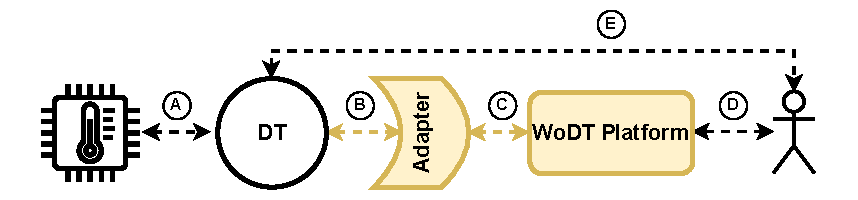
\includegraphics[width=0.8\columnwidth]{figures/hwodt/HWoDT-latency.pdf}
  \caption{Latency in an HWoDT-based system.}
  \label{fig:latency-hwodt}
\end{figure}

Accordingly, the following evaluation assesses the performance of the \ac{HWoDT} platform prototype, thereby characterizing the overhead incurred when integrated atop existing interoperability standards.
Even though performance optimization was not a primary focus in the development of the \ac{HWoDT} platform prototype, it can still be useful to make some considerations on the performance of the \ac{HWoDT} approach.
%
To do so an experimental setup is used to measure the latency \circled{B}+\circled{C}+\circled{D} when interacting with the platform and compare it with \circled{E}.

%-----------------------------------
\subsection{Experimental Setup}
%-----------------------------------

The experiment is designed to stress the performance of the platform in a resource-intensive scenario, and measure the delay perceived by consumers wishing to interact with \acp{DT} and the ecosystem as a whole.
%
A synthetic workload is used because---differently from a real-world \ac{IoT} dataset which may include data spikes over time---the scenario allows us to have a fully controllable environment to scale the traffic and evaluate the response of the platform under different loads.

A \ac{DTE} of a network of temperature sensors is implemented, with \acp{DT} reporting an update every second using \acp{DT} implemented with the \ac{WLDT} framework, running within the same process.
%
Each \ac{DT} generates a random temperature value between 0 and 100 every second, with a random initial offset of up to one second to avoid perfect synchronization of the \acp{DT}' data streams. The \ac{DT} state includes a timestamp marking when the state was computed by the \acp{DT}.
%
The different interaction patterns of the \ac{DTE} are tested:
\begin{itemize}
    \item with clients \emph{observing} all the \acp{DT} receiving all the \acp{DT} state notifications;
    \item with clients periodically \emph{querying} the \ac{DTE} to retrieve all sensors that have a reported temperature greater than 50. 
\end{itemize}
%
The key metrics collected are the \emph{freshness} of the information, which is computed as the difference between the time a state notification is received and the timestamp of the message (or the greatest timestamp when observing the \ac{DTE} \ac{KG}).
%
Additionally, the time taken to perform a query on the ecosystem retrieving the state of all \acp{DT} matching a condition is measured.

The experiments have been carried out running the \acp{DT} the \ac{WoDT} platform and the client applications on the same machine equipped with a 13th Gen Intel(R) Core(TM) i7-13700H CPU and 32 GB of RAM, using the OpenJDK 21.0.7 runtime.
%
Data is collected by analyzing logs of the client applications.

All \acp{DT} have been implemented with the \ac{WLDT} framework. 
The framework supports defining \ac{DT} implementations and uses a plugin-based architecture to expose different interfaces. 
This has been useful to implement different interaction patterns for the same \ac{DT}.

Measurements are repeated with 50, 100 and 200 \acp{DT}, and performing operations with 1, 50, 100 clients each observing all \acp{DT} and querying the entire \ac{DTE}.


%-----------------------------------
\subsection{Results}
%-----------------------------------

This section briefly reports results of the performance evaluation focusing on the different interaction patterns of the \ac{WoDT} platform prototype and comparing them with baseline direct interactions with individual \acp{DT}.
%
The results are summarized in \Cref{fig:sequence-interactions}, showing two bar plots reporting the average values of the two metrics collected in the experiments.
%
Results confirm that the overhead introduced by the \ac{HWoDT} platform is not negligible, but still acceptable for many \ac{DT} applications, especially when considering the benefits of having a uniform interface to interact with heterogeneous \acp{DT}, especially when considering the ability to query the whole \ac{DTE} \ac{KG}.

\begin{figure}
    \centering
    \begin{subfigure}[t]{0.49\textwidth}
        \centering
        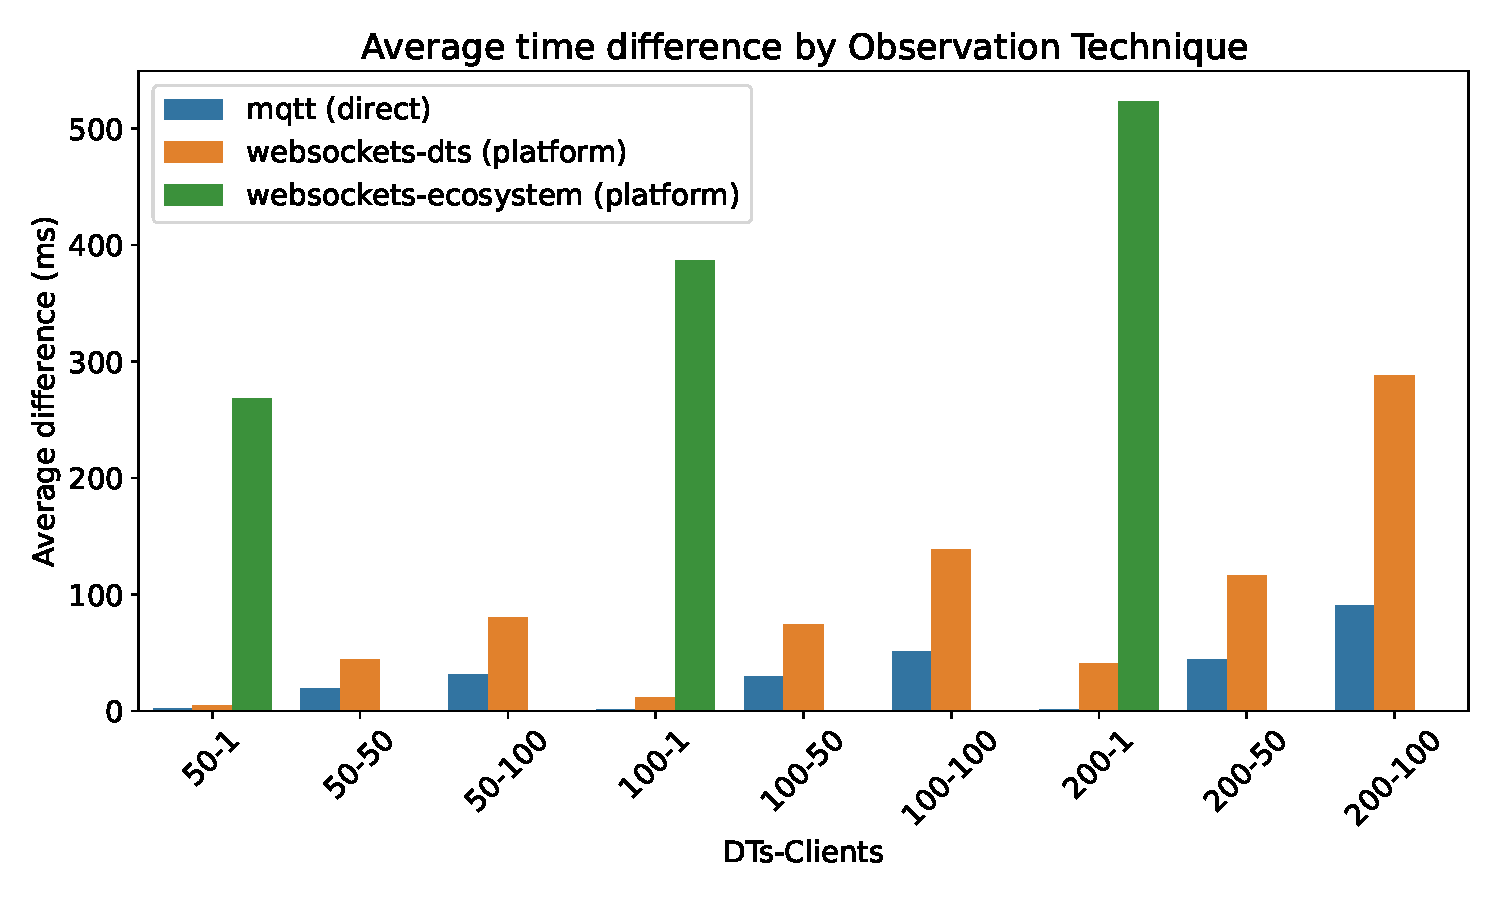
\includegraphics[width=\textwidth]{figures/hwodt/mean_latency_barplot.pdf}
        \label{fig:observation-delay}
    \end{subfigure}
    \hfill
    \begin{subfigure}[t]{0.49\textwidth}
        \centering
        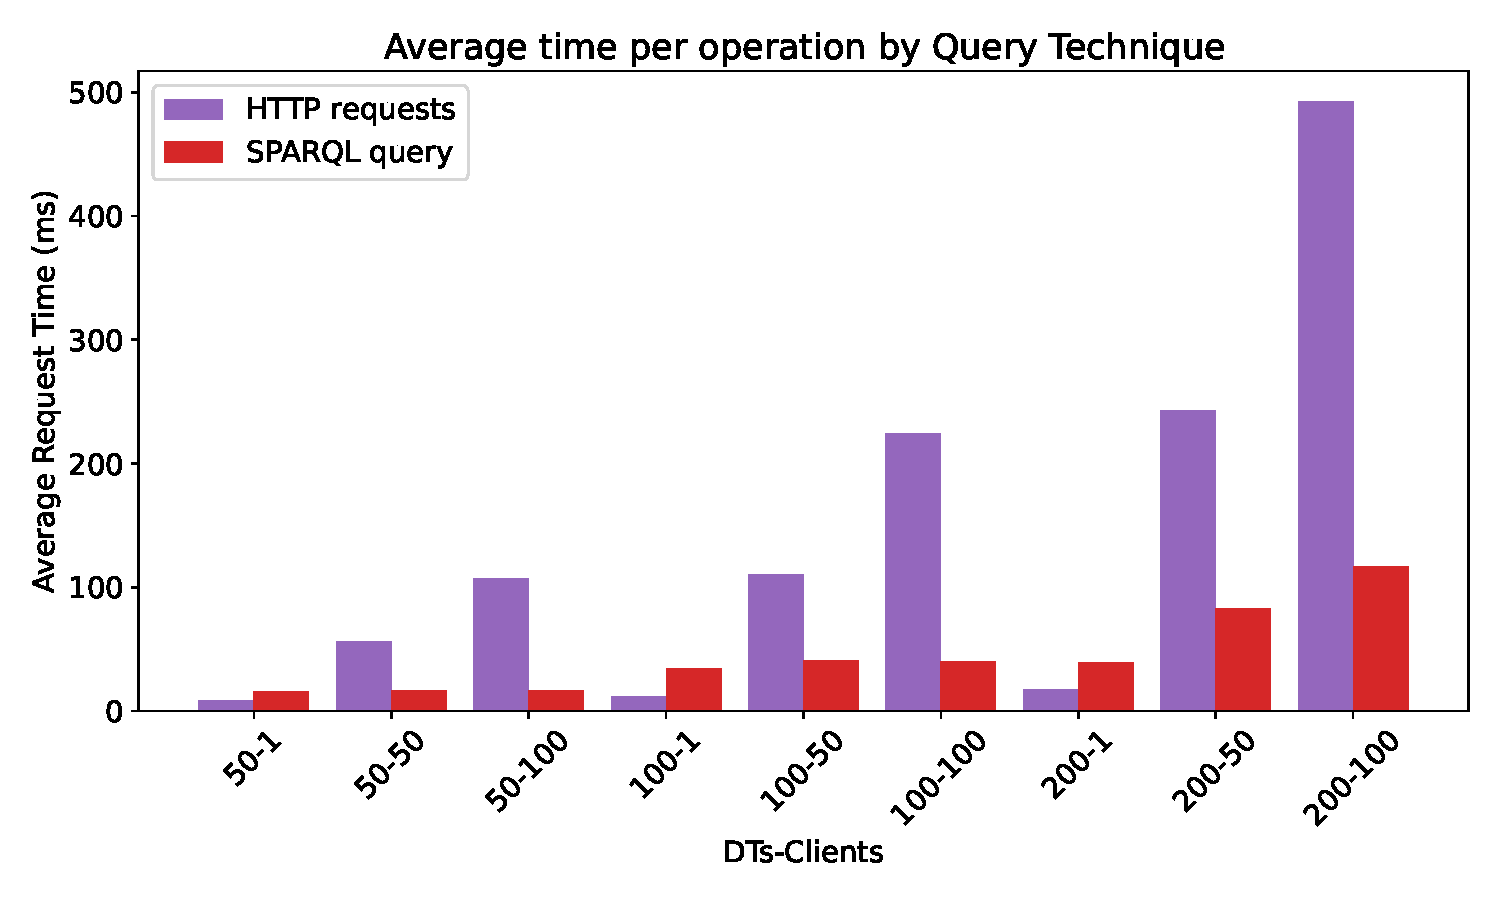
\includegraphics[width=\textwidth]{figures/hwodt/mean_request_time_barplot.pdf}
        \label{fig:query-time}
    \end{subfigure}
    \caption{Performance indicators with different loads of \acp{DT} and clients working on the ecosystem: (a) average time difference when observing \acp{DT} either directly or through the \ac{WoDT} platform, and (b) average time per operation when querying the DT ecosystem either through the \ac{WoDT} SPARQL endpoint or directly retrieving the state from each \ac{DT} API.}
    \label{fig:sequence-interactions}
\end{figure}

%...................................
\subsubsection{\aclp{DT} Observation}
%...................................

The \ac{HWoDT} adapter sends updates of the \ac{DTKG} on a WebSocket connection to the platform. Clients are set up to connect to the platform and observe each \ac{DT} through a WebSocket connection.
This aims to measure the delay introduced by the communication between the adapter and the platform, before getting to a final consumer. 
%
As the platform also supports observing the full \ac{DTE} \ac{KG}, a client also observes directly the \ac{KG} updates over a WebSocket connection (\circled{B}+\circled{C}+\circled{D}).
%
This is compared against direct observation of the \ac{DT}, which is implemented by sending each state update to an MQTT broker. Clients connect to all topics \texttt{dt/+/state} to observe all \acp{DT} (\circled{E}).

Whenever a message is received, the \emph{freshness} metric is computed as the difference between the timestamp of the message and the time the message is received using the system clock (which is synchronized as all processes run on the same machine). 
%
For the \ac{DTE} \ac{KG} as a new state update is generated for each change of each \ac{DT}, the greater timestamp among all \acp{DT} is taken to compute the freshness.

\Cref{fig:observation-delay} shows the average time difference with the different observation techniques. 
As expected, directly observing individual \acp{DT} is more efficient, as there is virtually no overhead. Users of the \ac{WoDT} platform should prefer this whenever possible, following the affordances of \acp{DT} in the \ac{DTD}.
%
In all scenarios, the delay grows with the number of \acp{DT}. This is especially evident when considering the observation of the whole \ac{DTE} \ac{KG}, which is the least efficient. Analyzing the performance of the prototype it was possible to deduce that this is caused by the serialization of the whole \ac{KG} to stream it at every update, which is computationally intensive. 
%
This is also the reason why the figure avoids reporting the observation of the ecosystem \ac{KG} with more than 1 client, as the results are significantly worse than the other options, even with just 1 client.
Performances are expected to be less drastically impacted when using smarter \ac{KG} update notification strategies---such as sending incremental changes (e.g., as in \cite{roffia2018fi})---at the cost of requiring more complex clients, capable of applying the changes to reconstruct the full state.

%...................................
\subsubsection{Repeated Querying}
%...................................

Clients can query the \ac{DTE} through the SPARQL endpoint of the \ac{WoDT} platform.
%
This is compared with performing an interrogation directly on all \acp{DT} to retrieve the current state and then filtering it on the client side which is implemented by having all \acp{DT} expose a simple HTTP endpoint \texttt{GET /state} to retrieve the current state of the \ac{DT} (similarly to what is shown in \Cref{fig:comparison-custom-vs-hwodt})
%
For each client, requests are sent every second, ideally, since \acp{DT} send updates at the same frequency, this would be a realistic way to monitor the sensor network in our scenario.

The overall time the operation takes is measured by computing the time of sending the request and the response for the SPARQL query, and the time of performing all HTTP requests and then filtering for the direct interaction.
The time of performing SPARQL queries (\circled{B}+\circled{C}+\circled{D}) is compared against the time taken by a client to perform an HTTP request to retrieve the state of each \ac{DT} and filter them on the client side \circled{E}.
%
\Cref{fig:query-time} shows that the average time taken to perform a query is significantly less than requesting the state on each \ac{DT}, especially when the number of \acp{DT} in the ecosystem grows. 
%
Notably, when running only 1 client, the overhead of the computation of the platform \ac{KG} makes using queries less effective. 

%...................................
\subsubsection{Remarks}
%...................................

Results indicate that, with large numbers of \acp{DT}, using SPARQL queries becomes a more scalable and effective approach for observing the evolution of the ecosystem over time, comparable with direct observation of all \acp{DT}.
%
While this approach may not capture every individual update from each \ac{DT}, it reliably provides the latest available state at the time of each query.
In this experimental setting, for instance, querying every second is realistically sufficient to capture almost all updates, as the client would match the update frequency of the sensors.
This trade-off favors scalability and responsiveness, especially in dynamic settings where maintaining subscriptions for all \acp{DT} would be resource-intensive or impractical.

The centralized implementation of the platform makes it a potential bottleneck. Specifically, interacting with the \ac{DTE} KG is costly because the graph gets updated by all \acp{DT} updates.
%
This is a reasonable trade-off as interacting with the \ac{DTE} provides advanced functionalities that would be impossible or very difficult to replicate simply by interacting with individual \acp{DT}.
%
Nevertheless, it will be interesting to explore optimization techniques for future improvements of the platform, as well as decentralized approaches to provide ecosystem services that would make the system less reliant on the platform itself.

% %=================================================
% \section{Discussion, Limitations and Future Works}
% %=================================================


%==============================
\section{Final Remarks}
%==============================

This chapter presents a proposal for the engineering of heterogeneous \acp{DTE} grounded on principles and technologies from the Web and the Semantic Web.
%
The chapter addresses the research question:

\paragraph{\ref{rq:2} How can we engineer DTEs that integrate heterogeneous DTs and support
applications in interacting with them?}
%%
The proposal of the \ac{HWoDT} addresses the challenges of integrating heterogeneous \acp{DT} by means of a uniform self-described interface that allows the representation of \ac{DT} interaction possibilities and metadata (through the \ac{DTD}) as well as the up-to-date state of the \ac{DT} (through the \ac{DTKG}).
%
The services and interfaces offered by the \ac{HWoDT} platform allow consumers to seamlessly interact with the \ac{DTE}, abstracting away the heterogeneity of the underlying \acp{DT}.
%
Consumers can either observe the evolution of the \ac{DTE} \ac{KG} or perform expressive queries to retrieve information through SPARQL. 
%
The prototype implementation of the \ac{HWoDT} platform and the set of adapters for representative \ac{DT} technologies demonstrate the feasibility of the approach in integrating \acp{DT} developed with different technologies through a shared semantic layer that can complement existing interoperability standards.
